\providecommand{\topdir}{..}
\documentclass[../main.tex]{subfiles}

\ifSubfilesClassLoaded{
  \externaldocument[main-]{../main}
  \setcounterref{chapter}{main-chap:conclusion}
  \addtocounter{chapter}{-1}
}{}

\externaldocument{\subfix{../00_front_matter/front_matter}}
\externaldocument{\subfix{../01_introduction/introduction}}
\externaldocument{\subfix{../02_lorenz96/lorenz96}}
\externaldocument{\subfix{../03_rayleigh_benard/rayleigh_benard}}
\externaldocument{\subfix{../04_tendencies/tendencies}}
\externaldocument{\subfix{../05_evaluation/evaluation}}
\externaldocument{\subfix{../07_appendix/appendix}}

\begin{document}

\ifSubfilesClassLoaded{
    \frontmatter
    \tableofcontents
    \mainmatter
}{}

\chapter{Discussion} \label{chap:conclusion}
\setlength{\epigraphwidth}{.45\textwidth}
\epigraphhead[0.1\textheight]{
    \epigraph{
        God does not care about our mathematical difficulties; He integrates
        empirically.
    }{
        Albert Einstein, quoted by Leopold Infeld in
        \emph{Quest: an autobiography}, 1941
    }
}
\todo{introductory paragraph}
In \crefrange{chap:rayleigh_benard}{chap:evaluation}, I presented a
complete proof of concept for data-driven parametrisation in \rb{} convection,
from the initial formulation of the problem to the assessment of the
parametrised model in an online setting. In the final chapter of this thesis, I
will discuss in greater detail the main obstacles that were encountered in the
process (\cref{sec:issues}) and the concrete outcomes of this work
(\cref{sec:outcomes}) before drawing final conclusions in
\cref{sec:conclusion}.


\section{Practical issues and their implications} \label{sec:issues}
This work has highlighted several obstacles to the practical implementation
data-driven parametrisation that were initially not obvious from a purely
theoretical point of view or not applicable to earlier work using simpler
dynamical systems such as Lorenz '96. Fundamentally, many of these arise
because the \rb{} problem is spatially continous---a PDE, as opposed to ODEs
like Lorenz '96.


\section{Coarse model instability}
One of the earliest issues encountered in this work was the potential for
low-resolution models to become numerically unstable, making it difficult to
obtain a baseline for evaluating parametrised models. Aside from the need for
a baseline, it seems unlikely that a simple parametrisation scheme like the one
developed in \cref{chap:tendencies} would have improved the skill of a
coarse model on the brink of instability. Since this work was not concerned
with accurately representing physical reality, I chose to artificially add
hyperviscosity terms to the equations. Another option for future work could be
to use stress-free boundary conditions on the top and bottom plates (i.e.,
$w(z=0,1) = \partial u/\partial z|_{z=0,1} = 0$) rather than the no-slip
condition. This could reduce the large near-wall temperature and velocity
gradients that often triggered instability at low resolutions.

However, when modelling real-world systems such as the atmosphere, one does
not have the freedom to simply alter the governing equations. Successful
data-driven parametrisation in these cases will depend on the careful choice of
the numerical methods used to discretise and solve the equations such that
the underlying coarse model is stable, even if it is inaccurate. Futher work
with the \rb{} system should investigate whether other types of solvers
(finite difference/volume/element, etc.) are more suitable.


\subsection{The coarse-graining problem}
The predictability of the subgrid tendencies was found to depend strongly on
the method used to coarse-grain the high-resolution solutions, and the
development of an an appropriate method was non-trivial. These findings
can be justified with further discussion.

The Lorenz '96 system \cref{eqn:l96} explicitly separates its degrees of
freedom into ``coarse'' and ``fine'' variables, allowing one to unambiguously
define a reduced model by simply truncating the fine variables from the full
model. The corresponding ``coarse-graining'' operation is trivial: just discard
the fine variables. For spatially continuous systems like \rb{}, however,
standard practice is to construct high- and low-resolution models independently
from each other by applying (possibly different) discretisation schemes to the
governing equations. Since the low-resolution model is not, in general,
obtained by explicitly truncating the high-resolution model, it is up to the
modeller to choose a coarse-graining operation that maps the high-resolution
state space to the low-resolution one. While instructive, Lorenz '96 and its
coarse/fine paradigm are not helpful analogues in this respect.

As explained in \cref{sec:coarse_graining}, it was essential for the
coarse-graining operation to smooth the high-resolution fields to make them
resolvable on the coarse grid. This requirement can be connected to the issue
of scale separation, which was discussed in \cref{chap:introduction} as
one of the main constraints on parametrisability. For a system whose energy
spectrum has clear scale separation, as sketched in
\cref{fig:scale_separation}a, a coarse model that cannot resolve the
high-wavenumber behaviour can still capture the low-wavenumber features with
good resolution (\cref{fig:scale_separation}b). Such a coarse model is
therefore likely to be numerically stable, and the system's parametrisability
relatively insensitive to the choice of coarse-graining operation; simple
averaging over each coarse grid-box will easily remove the high-wavenumber
fluctuations. On the other hand, a system lacking scale separation
(\cref{fig:scale_separation}c) presents a far greater challenge because
coarse-graining with insufficient smoothing will leave too much power at the
highest wavenumbers resolvable by the coarse model (darker blue dots in
\cref{fig:scale_separation}d), leading to numerical instability.

Future work must be mindful of the technicalities surrounding coarse-graining,
especially for systems like \rb{} that lack scale separation. The approach
used in this work has shown promise and could continue to be a useful tool.
\todo{any literature?}

\begin{figure}[ht]
    \centering
    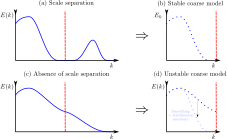
\includegraphics[width=0.7\linewidth]{figures/scale_separation.pdf}
    \caption{
        \textbf{(a):} Cartoon sketch of the energy spectrum for a system that
        exhibits clear scale separation. \textbf{(b):} The likely discrete
        energy spectrum of a coarse model of the system in (a), corresponding
        to a well-resolved and numerically stable solution. \textbf{(c-d):}
        Counterparts of (a-b) for a system lacking scale separation,
        resulting in a poorly-resolved and numerically unstable coarse solution
        solution unless action is taken to stabilise the model and apply
        smoothing when coarse-graining.
    }
    \label{fig:scale_separation}
\end{figure}


\subsection{Subgrid tendency modelling}
% § Alternative approaches in literature (Alieva, Gentine papers)
Another obstacle to data-driven parametrisation for spatially continuous
problems is that there is a very large number of possible subgrid tendency
predictors. For \rb{}, one not only has the three prognostic variables, but
also their derivatives to arbitrary order in the two spatial directions. The
position-dependence of the subgrid tendency statistics was a further
complication, adding $z$ to the list of predictors. One could even use
spatially or temporally nonlocal predictors (i.e., the values of the variables
at nearby points in space or previous time steps)---a possibility that was not
even considered in this work. It would be impossible for a human to explore
every possible combination. Supervised machine learning algorithms, discussed
briefly in \cref{sec:data_driven}, are much better-suited to regression
problems with large numbers of predictors and could potentially capture hidden
and/or nonlinear relationships between these predictors and the subgrid
tendencies. There is no doubt, however, that this work was limited by the
simplicity of the predictors and regression models that were considered, and
future work using more sophisticated statistical models may indeed have greater
success without needing to resort to machine learning.

This work was further limited by its use of purely deterministic
parametrisation schemes despite the existence of considerable residuals
in the subgrid tendency regressions
\crefrange{fig:theta_subgrid_vs_pred_tend}{%
fig:w_subgrid_vs_pred_tend}. Stochastic parametrisation, discussed in
\cref{sec:stochastic}, has the potential to reduce mean-state model
biases by emulating the observed residuals. With the tools I have developed for
the \rb{} problem, it would be relatively straightforward to experiment with
various stochastic perturbations of the existing deterministic scheme
\cref{eqn:scheme}, beginning with those that have been tested for
Lorenz '96 (see \cref{sec:l96_statmodels}). This would include the use
of time-correlated (e.g., AR(1)) noise to reflect the persistence (memory)
of the subgrid tendencies.


\section{Outcomes and opportunities for future work} \label{sec:outcomes}
\subsection{Subgrid tendency correlations}
% ○ There is evidence that subgrid tendencies are still predictable from the large-scale state
% ○ Resolved tendency correlation
%   § Insufficient dissipation - paper
%   § Convection causes converging moisture to rain out
The joint histograms shown in \cref{chap:tendencies} clearly show that the
subgrid tendencies are predictable given the coarse state.


\subsection{Online performance}
% § Data-driven works
% § Good forecast and climate --> science question


\subsection{Framework and tools for future research}
% § Reproducibility, readability
% § Capabilities


\subsection{Unanswered questions}
% ○ Address goals that were not achieved, how they might be addressed using tools developed here
% § Assess value added by stochasticity and memory
%     ○ And the way in which they are added - e.g. additive vs. multiplicative noise, spatially/temporally correlated vs. white noise
% § Relationship between offline correlation and online performance
% § Relationship between short-term forecast skill and long-term statistics


\section{Conclusion} \label{sec:conclusion}
% ○ Developed an understanding of the practical issues involved in data-driven parametrisation
% ○ Methods from L96 do not easily generalise to real fluid models
% ○ Successful proof of concept and concrete tools for further research

% much to be learned

\ifSubfilesClassLoaded{%
    \emergencystretch=5em
    \printbibliography{}
}{}

\end{document}
